% Please do not change the document class
\documentclass{tufte-handout}

% Please do not change these packages


% You may add additional packages here
\usepackage{amsmath}
\usepackage{graphicx}
\usepackage{wrapfig}
\usepackage[rightcaption]{sidecap}
\graphicspath{ {../images/} }

% Please include a clear, concise, and descriptive title
\title{Mad Mechs Handout} 



\author{1507516}

\begin{document}

\maketitle


\section{Overview \& High concept}
Mad Mechs is a turn based strategy game featuring giant Mechs.
The game will feature a number of different systems, such as a in-depth customization system, detectable buildings and different factions.
The customization system will allow players to create a mech from a wide variety of parts. Each section can be equipped with a light, medium or heavy part. There will also be a large selection of different types of weapons that the mech can use.
The games aesthetic is a cell shaded borderlands style game, with cartoon style particle effects. 

\begin{figure}[h]
	\caption{The template for the mission selector}
	\centering
	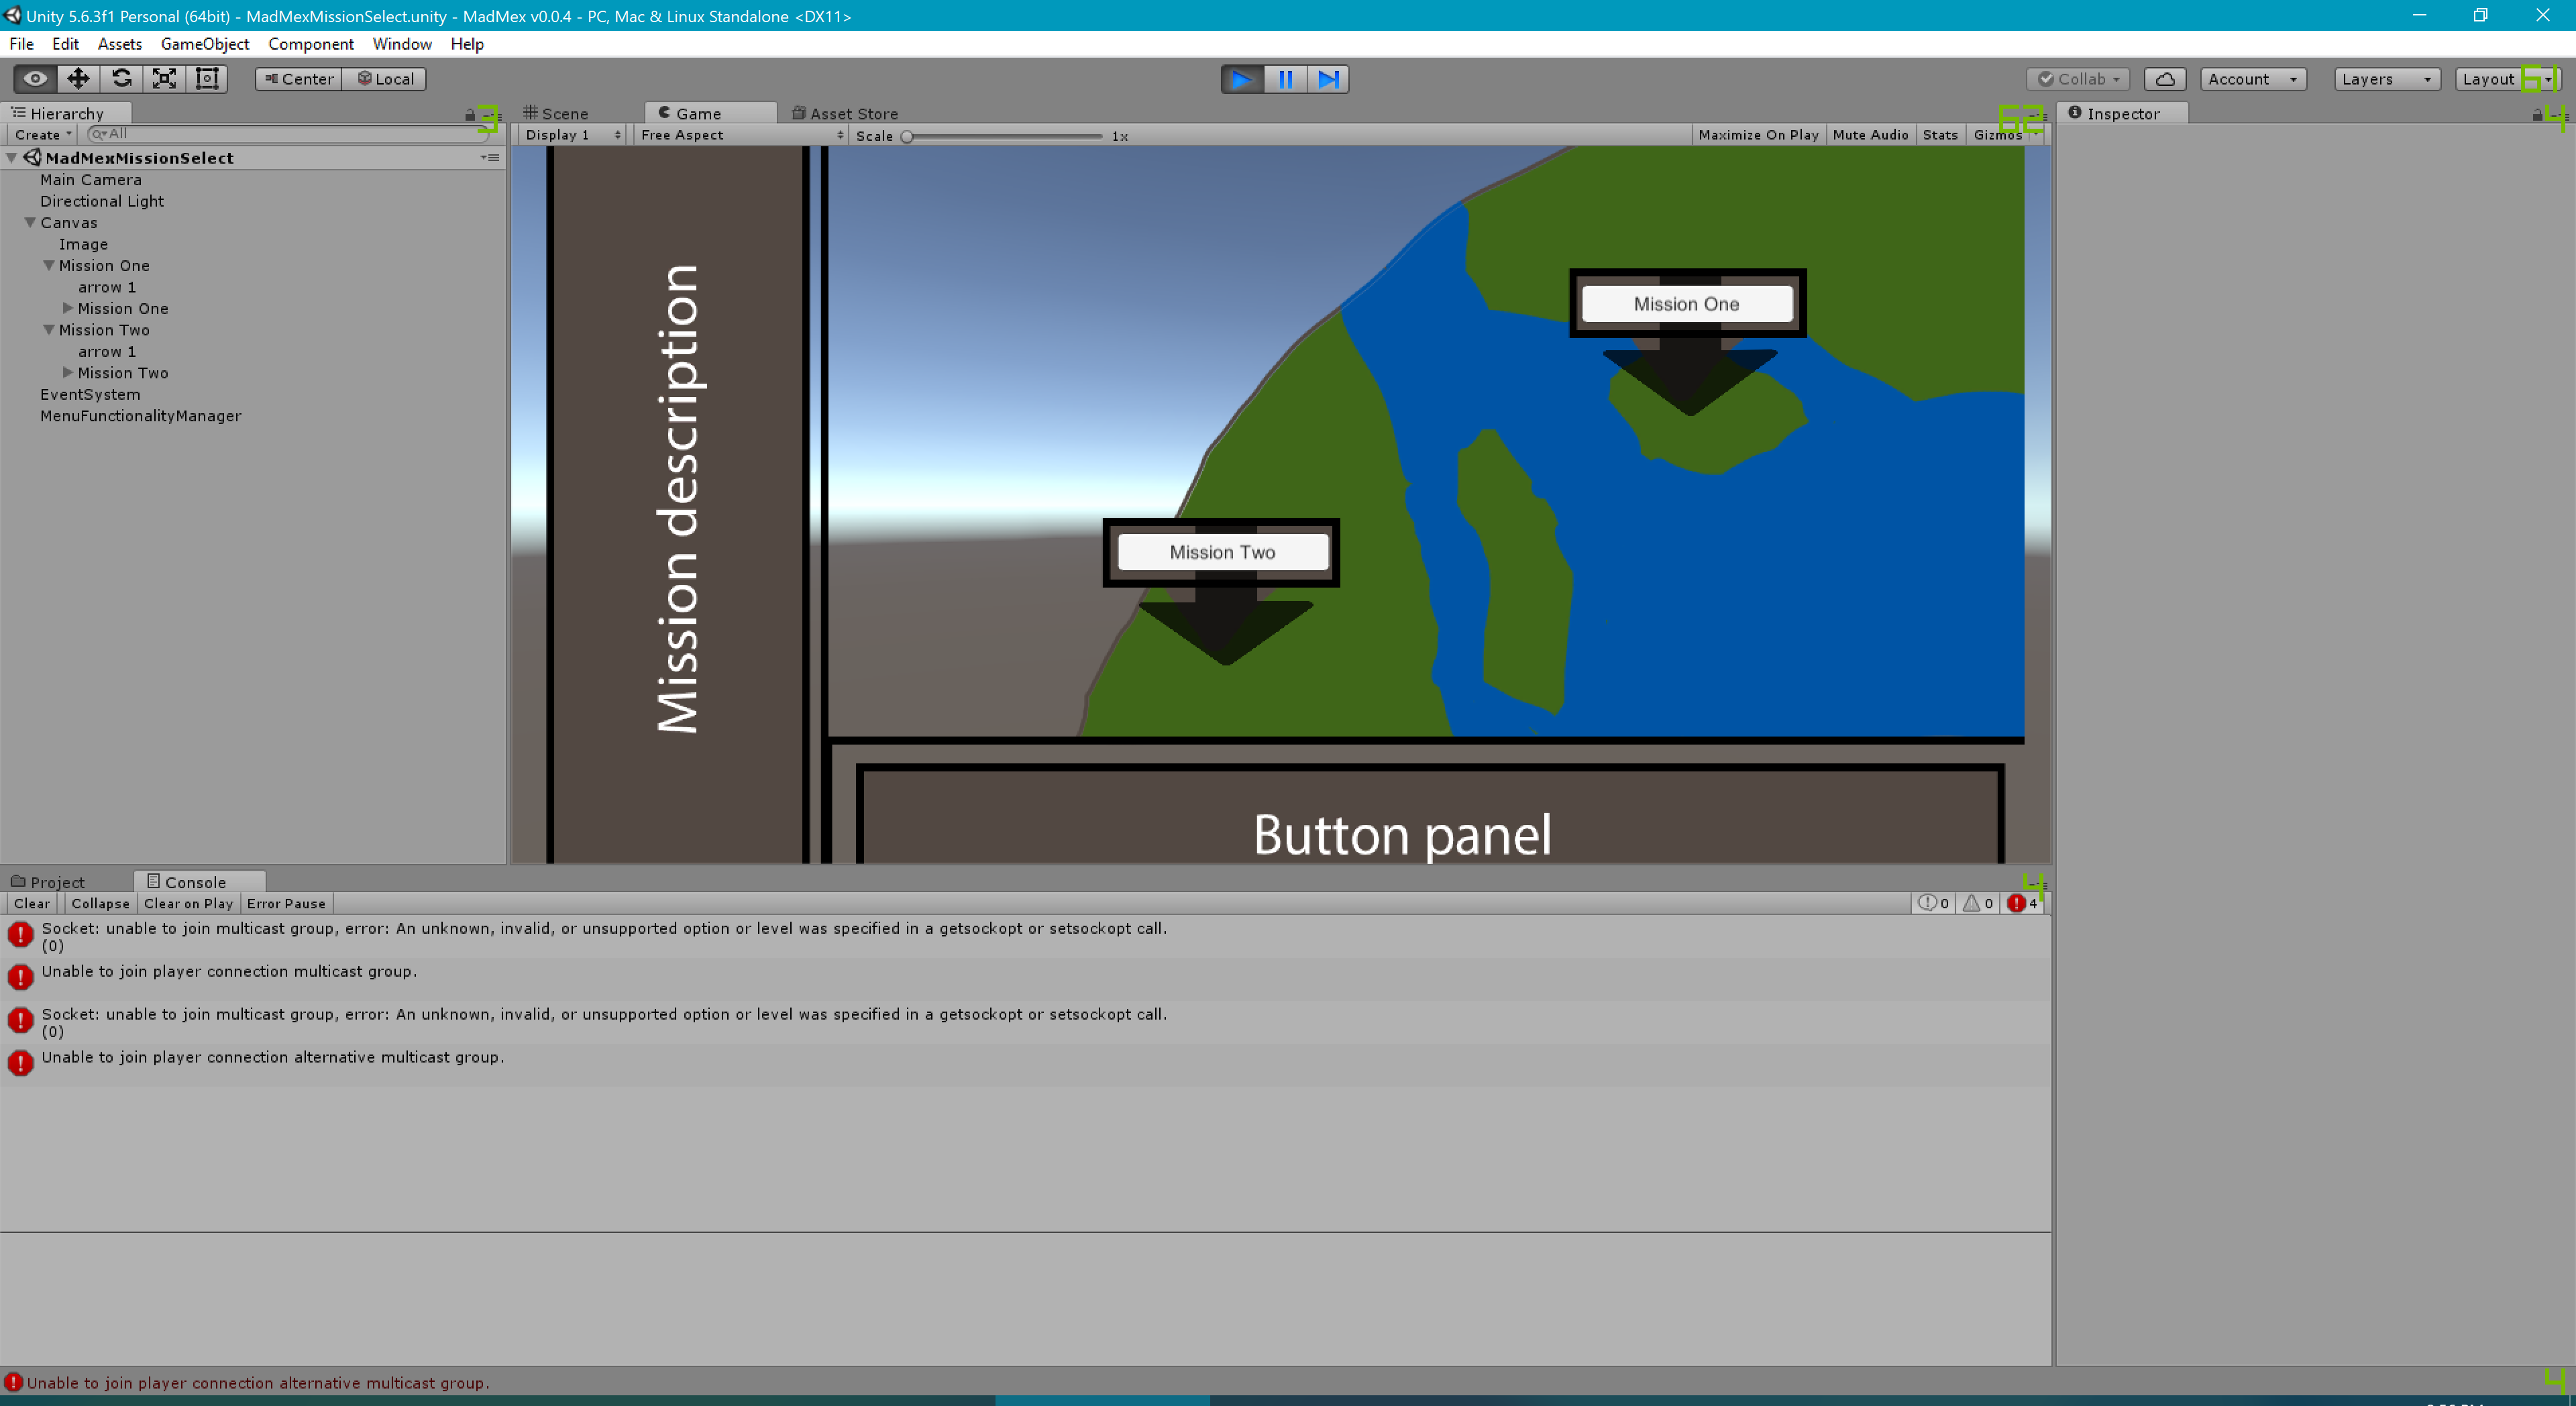
\includegraphics[width=0.8\textwidth]{MissionSelect}
\end{figure}

\section{Technical Feasibility}
Currently most of the core components of the game are almost all there. There is a basic test level that contains building destruction, mech customization, cell shading, basic AI and Action Point based combat on a grid. 
The player is given a set amount of action points, which is determined by the loadout of their mech, i.e. if they have a heavy or light mech. Light mechs will have a larger amount of movement and less HP where as, heavy mechs will have more HP and weapon damage and less movement.


\begin{figure}[h]
	\caption{Basic cell shading within the test build, it isn't very clear because none of the models have been textured yet.}
	\centering
	\label{testBuild}
	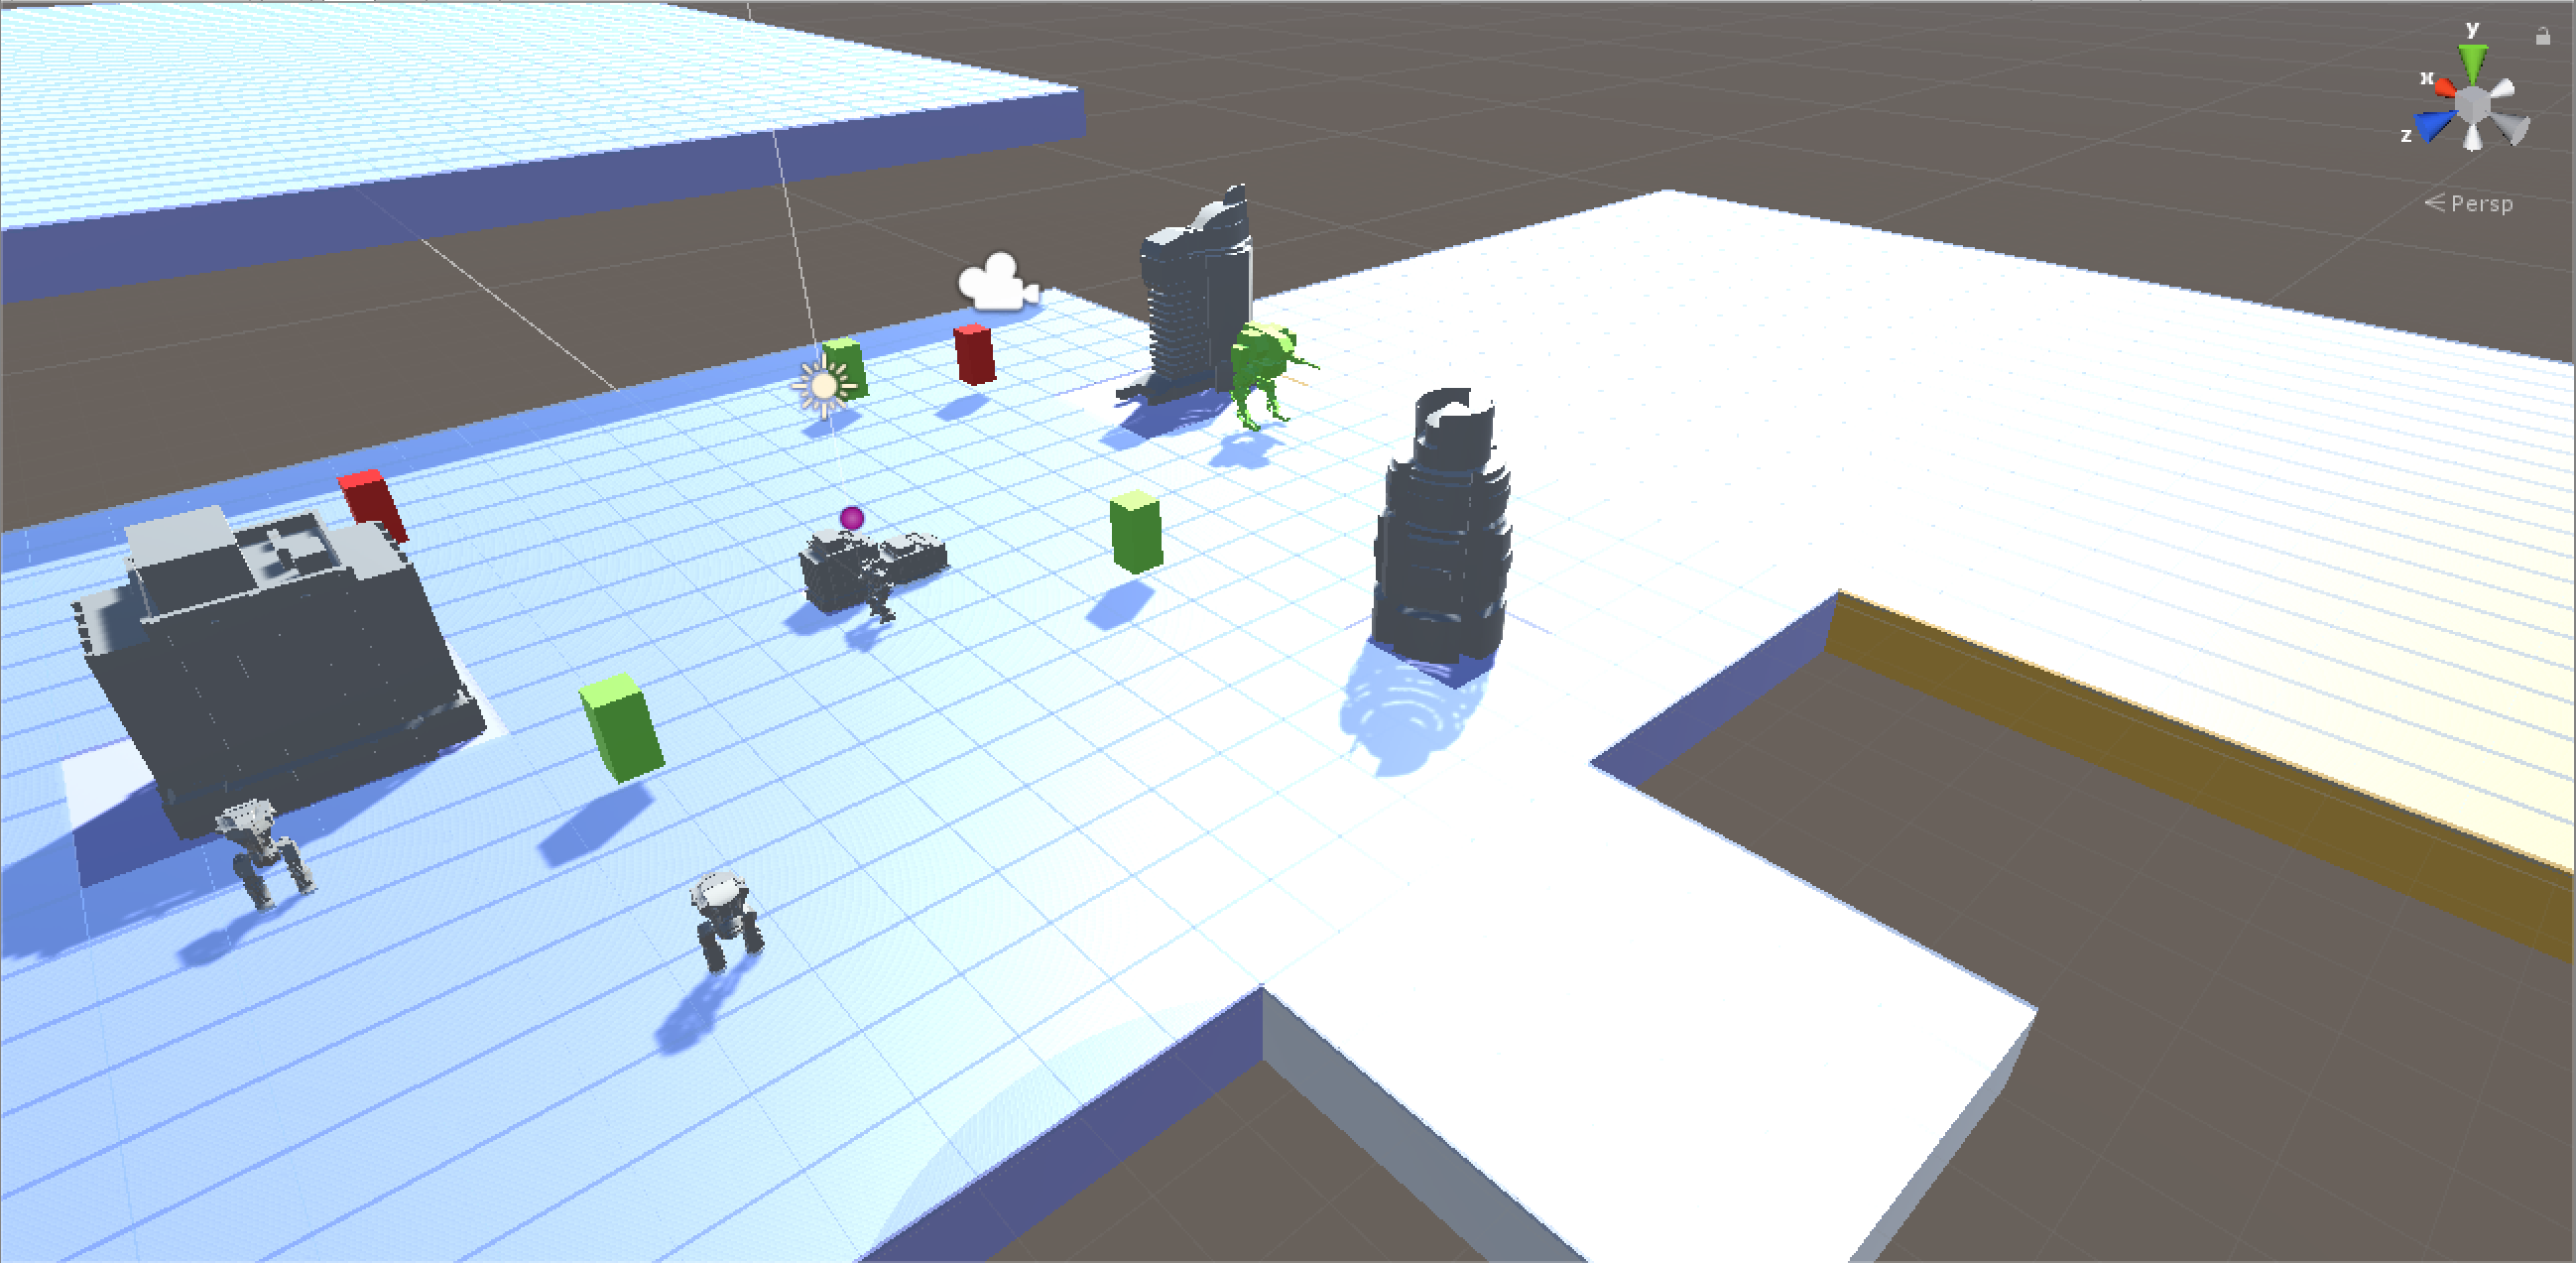
\includegraphics[width=1.0\textwidth]{TestBuild}
\end{figure}

Moving forward there will be edge detection to add to help emphasize the cartoon style of the game.

There is a grid of tiles that are generated on any game object, which creates a grid of tiles that the player can move the mech on. Furthermore it does not create tiles on the gameobject when there is buildings placed on it. This will allow for quick iteration of game levels when the necessary assets get added. This grid can be shown in figure \ref{testBuild}.

\section{USP}
A title that is a large source of inspiration for this  game is XCOM series. The games are very popular on steam and have had over 1.8M sales according to steamspy.
Another similar style game is Invisible, Inc.

The target audience for this game are people who enjoy turn based strategy games, aged 18-40.

\begin{figure}[h]
	\caption{The five different factions within the game, each one with a different aesthetic and types of mechs.}
	\centering
	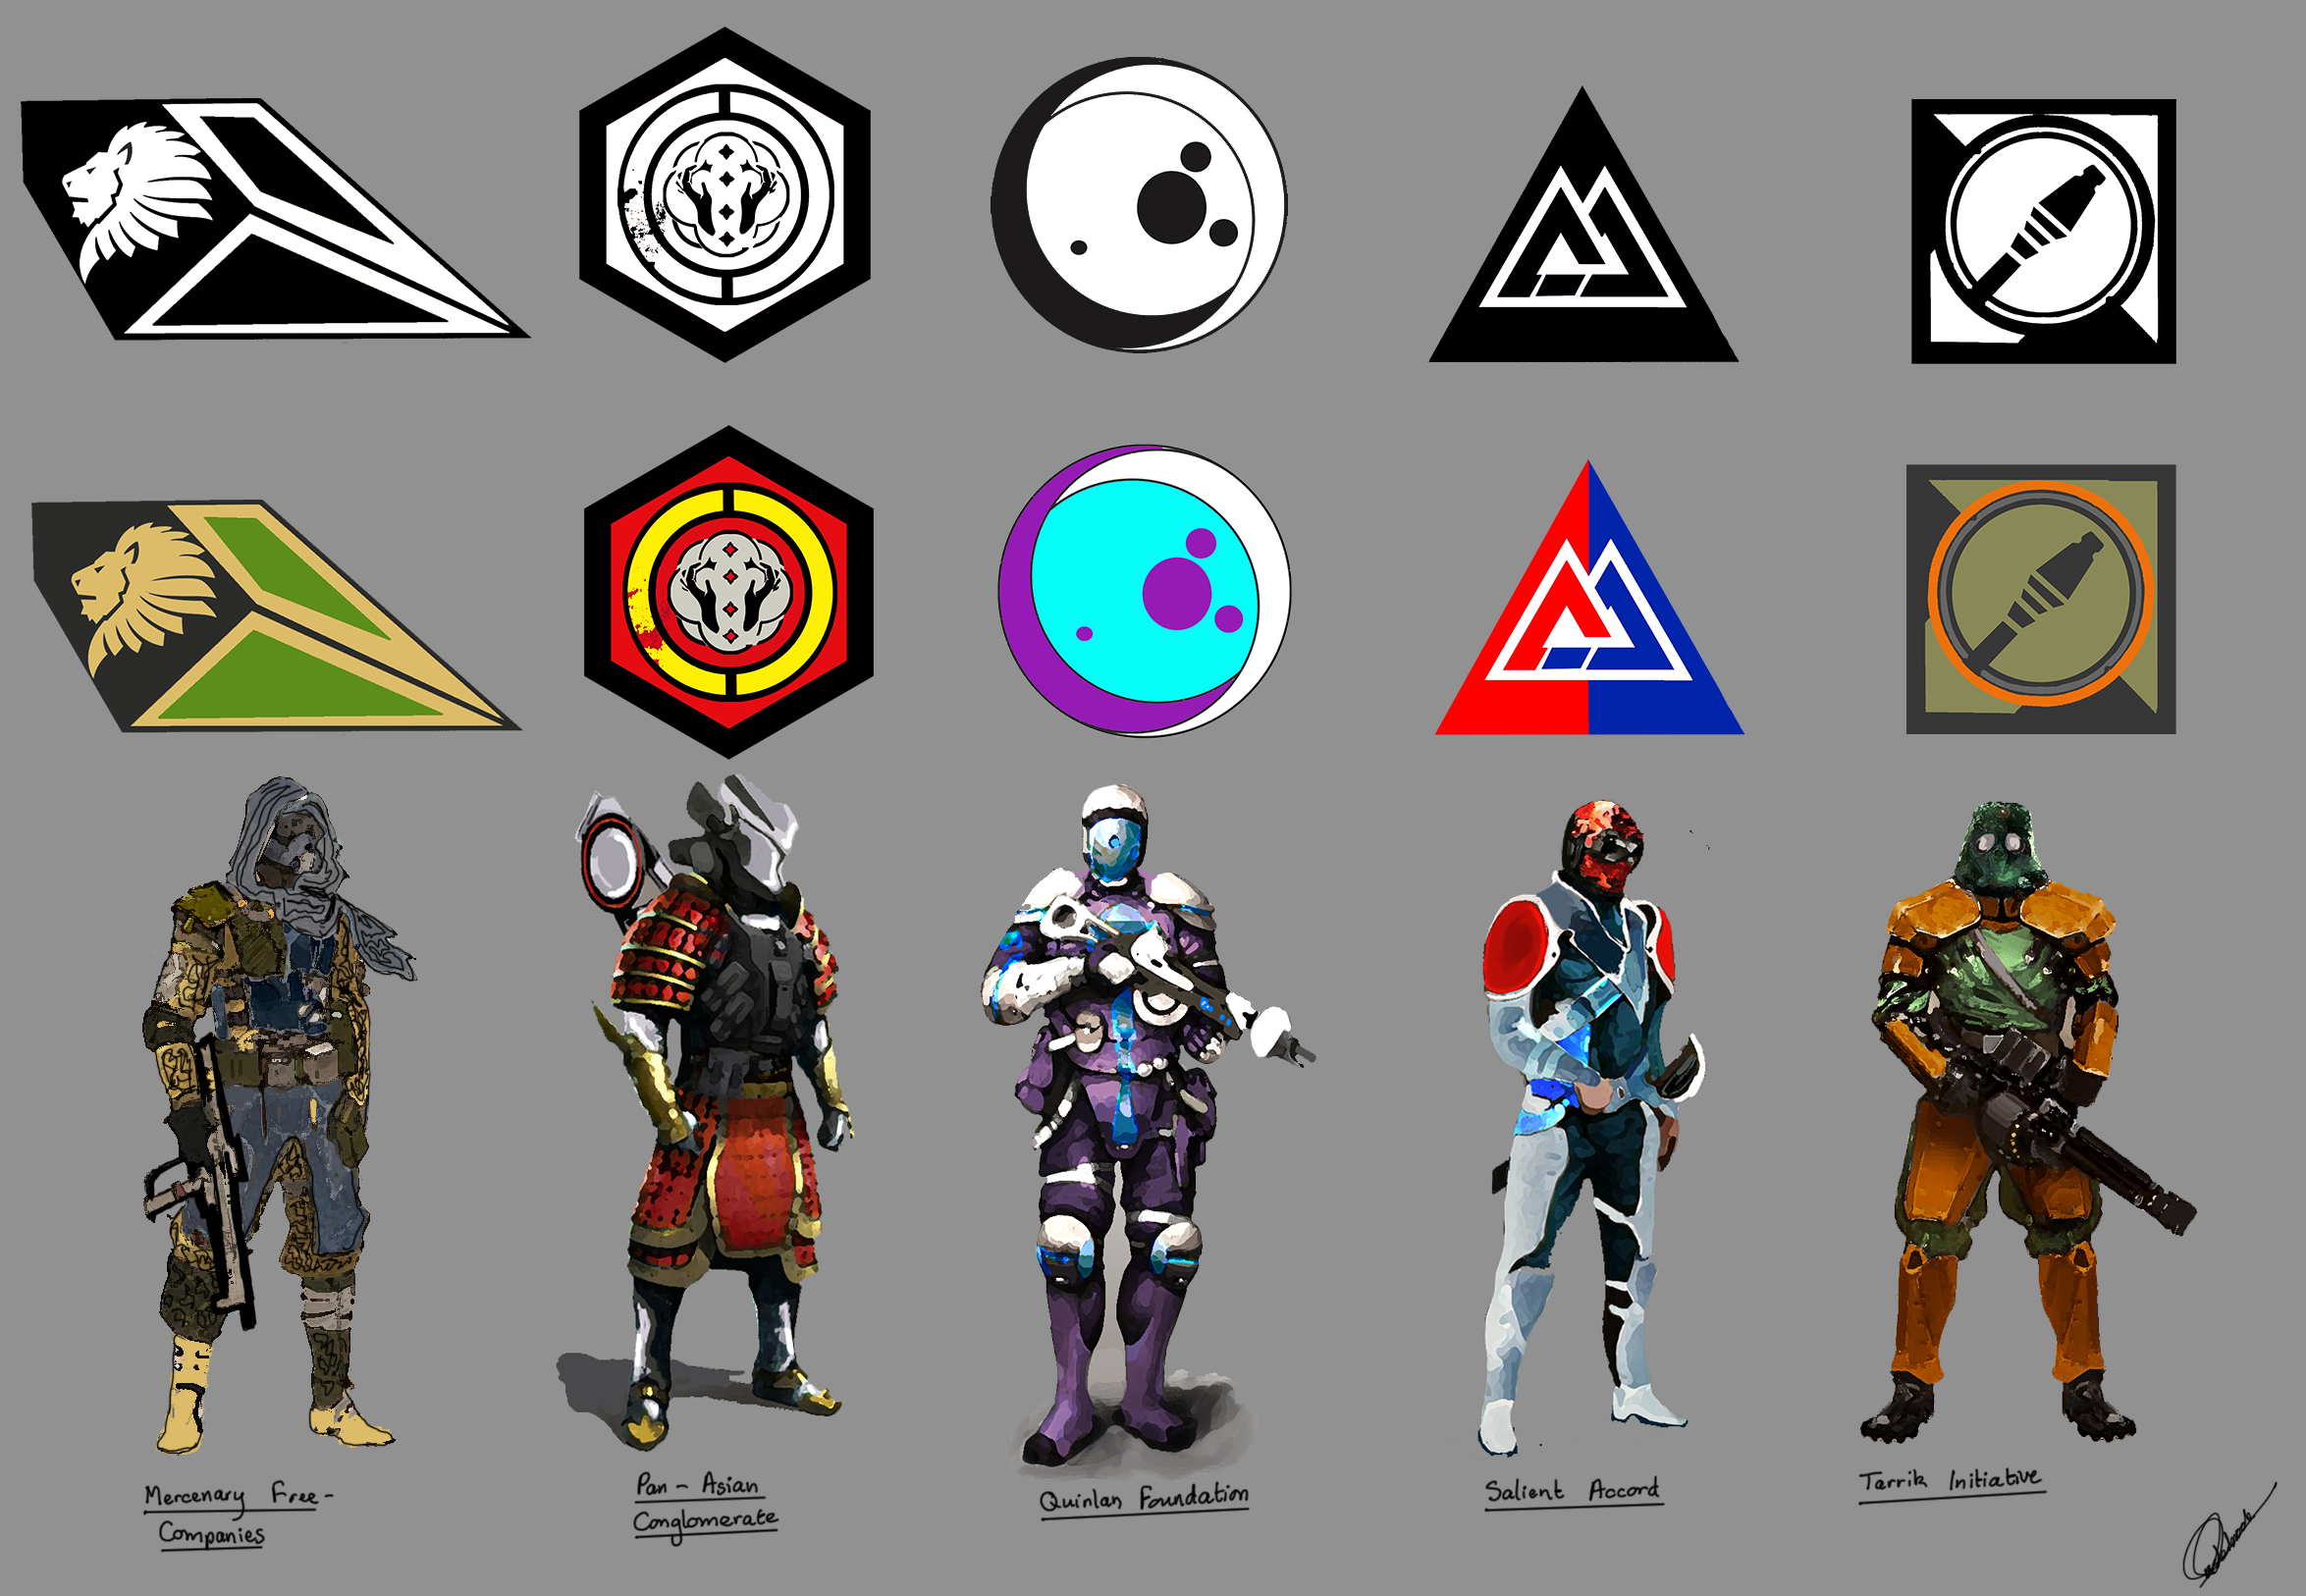
\includegraphics[width=0.8\textwidth]{factions}
	\label{factions}
\end{figure}

The unique selling point for this game is its detailed mech customization and the scale of the game. Furthermore the game has a unique building destruction system that will allow players to create a domino effect with buildings.

There will be at least 5 different factions within the game, each with a different backstory as shown in figure \ref{factions}. 


\end{document}


